\section{A complete operator with many defects}
\label{op:section}

We now choose one endomorphism of $\widehat T'$ from the operation
algebra of Proposition~\ref{complete:operations}, using finite matrix
blocks on Laurent series to control its action on the overlap. The
construction also keeps a prescribed reduction on the closed chart,
which the obstruction argument will use after gluing. Integral
interpolation measures from the group action let us control successive
matrix depths; a choice of base-$p$ digits then determines which rows
and columns remain unmatched.

Retain the chart action of Proposition~\ref{geom:thickened-charts}, the digit
filtration of Lemma~\ref{geom:group-filtration}, and the complete operation
algebra of Proposition~\ref{complete:operations}. Thus
\[
 k=\F_{p^2},\qquad R=k[[x]],\qquad
 \Delta=R[[H]],\qquad \mathscr E_0=\Delta^\Lambda.
\]
The initial symbol of $U_3=\delta_\gamma-\delta_1$ in the weight filtration
of Proposition~\ref{geom:skew-filtration} is $C$; the weights of $x$ and $U_3$
are respectively $4$ and $3$. Here $\delta_g$ denotes a Dirac measure,
and $1$ denotes the identity of $H$.

Put
\[
 K_0=k((x)),\qquad w=x^{-q},\qquad
 \Phi=K_0^\Lambda=k((w^{-1})).
\]
The subscript in $K_0$ refers to this Laurent field, not to Morava
$K$-theory.

Give $\Phi$ its Laurent-series topology, with standard compact open
subspace $k[[w^{-1}]]$. We seek one operator $a\in\mathscr E_0$ with
closed image and two fixed families: nonzero kernel series in
$k[[w^{-1}]]$ with distinct leading positions, and classes of positive
monomials $w^j$. The leading position of a nonzero series is the
greatest exponent of $w$ occurring in it. For fixed constants $c>0$
and $\beta>1/3$, which may depend on $p$, and every sufficiently large
integer $N$, at least $cN^\beta$ leading positions from the first
family should lie in $[-N,0]$, while at least $cN^\beta$ of the
selected classes with $1\le j\le N$ should be independent in
\[
 \Phi\big/\bigl(a\Phi+k[[w^{-1}]]\bigr).
\]
The first family lies in the compact subspace, while the second remains
independent after quotienting the cokernel by the image of that
subspace. Proposition~\ref{op:operator} supplies matrix conditions,
and Section~\ref{glue:section} proves that they yield these analytic
properties.

For $g\in H$ define
\begin{equation}
 z_g=\frac{g(x)}x,\qquad h_g=\frac{g(w)}w=z_g^{-q},
 \qquad u_g=h_g-1.
 \label{op:displacements}
\end{equation}
Both $z_g$ and $h_g$ belong to $1+xR$. Since $q$ is prime to $p$,
\[
 \ell(g):=\operatorname{ord}_x(u_g)
       =\operatorname{ord}_x(z_g-1),
\]
where the value $\infty$ is allowed. For $l\ge1$ let
\[
 H_l=\{g\in H:\ell(g)\ge l\},\qquad N_l=[H:H_l].
\]
These are the normal open congruence subgroups given by the action on
$R/x^{l+1}$. Since the action preserves valuation, the distance between
$z_g,z_{g'}$, and also between $u_g,u_{g'}$, has valuation
$\ell(g^{-1}g')$.

\subsection{Displacement and interpolation measures}

The next bound relates the digit filtration of $H$ to the rate at
which distinct orbit points approach one another. It has two uses.
Here it bounds the denominators of divided differences, so that
interpolation produces measures in $\Delta$. In the obstruction
argument, the same estimate will bound joint operator kernels.

\needspace{16\baselineskip}
\begin{lemma}[Displacement bound]
\label{op:displacement}
If $g\in H(i)\setminus H(i+1)$, then
\begin{equation}
 \ell(g)\le r_i:=\sum_{j=1}^i p^{\lfloor j/2\rfloor}.
 \label{op:digit-displacement}
\end{equation}
The action of $H$ on $R$ is faithful. With $r_0=0$, one has
\begin{equation}
 \kappa:=\sum_{l\ge1}\frac1{N_l}\le\frac p{p-1}.
 \label{op:kappa}
\end{equation}
Moreover, for every $s\ge1$,
\begin{equation}
 \Gamma_s\subset H_{p^s}\subset H(2s-1),
 \qquad N_{p^s}\ge p^{3(s-1)}.
 \label{op:congruence-index}
\end{equation}
\end{lemma}

\begin{proof}
We first bound the displacement of an element from its first
nonidentity digit. The comparison is made on torsion points of the
deforming formal group, where the digit gives an exact valuation
and the displacement gives a lower bound for the same expression.

Choose a strict representative of $g$ whose first nonidentity digit is
at index $i$, with coefficient $b\ne0$. For even $i$, choose
$b\notin\F_p$, using the quotient by the central subgroup. The chart
construction gives a formal isomorphism
\[
 \widetilde g:F_y\longrightarrow F_x,\qquad y=g(x),
 \qquad [p]_{F_x}(T)=xT^p+_{F_x}T^{p^2}.
\]
Its coefficients lie in $R$: the grading change is effected by a
$(p-1)$-st root congruent to $1$, followed by the compatible strict
arrow. The reduction of $\widetilde g(T)-_{F_x}T$ begins with
$bT^{p^i}$.

Extend the valuation $v(x)=1$ to a completed algebraic closure of $K_0$.
Formal group series over $R$ can be evaluated on its positive-valuation
ball. The zeros of $[p^d]_{F_x}$ in this ball form a cyclic group of order
$p^d$, and every zero has multiplicity $p^d$. Indeed, Weierstrass
preparation, using reduction $T^{p^{2d}}$, gives a polynomial of degree
$p^{2d}$ all of whose zeros reduce to zero; its unit factor evaluates to
a unit. The order at zero over $K_0$ is $p^d$. Translation by a torsion
point is an invertible formal coordinate change and preserves
multiplicity, so the group of zeros has order $p^d$. Its subgroup killed
by $p$ has order $p$, which proves cyclicity.

A primitive level-$d$ point $\zeta$ has valuation
\[
 \lambda_d=\frac1{(p-1)p^{2d-1}}.
\]
For $d=1$, the two summands of the $p$-series must have equal valuation.
Inductively, to have $v([p]\zeta)=\lambda_{d-1}$, one must have
$v(\zeta)<\lambda_1$; in that range the $p^2$-power summand dominates.
This proves the formula.

Fix $i$ and take $d$ sufficiently large. The residue of
\[
 \frac{\widetilde g(\zeta)-_{F_x}\zeta}{\zeta^{p^i}}
\]
is $b$: coefficients of lower powers of $T$ lie in $xR$, and their
valuations exceed $p^i\lambda_d$ for large $d$. The differences
$\tau-_{F_x}\zeta$, as $\tau$ ranges over the level-$d$ torsion points,
are the multiples $[a]_{F_x}\zeta$ for $a\bmod p^d$. If
$s=\nu_p(a)<d$, their valuation is $p^{2s}\lambda_d$; the zero multiple
has infinite valuation. When $2s=i$, the residue after division by
$\zeta^{p^i}$ is $a/p^s\bmod p\in\F_p^\times$, since
$[p^s]_{F_0}(T)=T^{p^{2s}}$. It cannot cancel $b$. Ordinary and formal
differences have the same valuation, because $T-_{F_x}S$ is $T-S$ times
a unit. Consequently
\[
 v(\widetilde g(\zeta)-\tau)=p^{\min(i,2s)}\lambda_d,
\]
with $s=\infty$ for $\tau=\zeta$.

There are $(1-1/p)p^{d-s}$ multiples of exact order parameter $s<d$.
Counting these factors with multiplicity $p^d$ in the Weierstrass
factorization gives
\begin{align}
 v\bigl([p^d]_{F_x}(\widetilde g(\zeta))\bigr)
 &=p^{2d}\lambda_d
   \left((1-1/p)\sum_{0\le s<\lceil i/2\rceil}p^s
                   +p^{i-\lceil i/2\rceil}\right)\notag\\
 &=\frac{p^{\lceil i/2\rceil}+p^{\lfloor i/2\rfloor+1}-1}{p-1}
   =r_i+\frac p{p-1}.
 \label{op:torsion-valuation}
\end{align}
On the other hand, substitution gives
$F_y\equiv F_x\bmod x^{\ell(g)+1}$. Since $[p^d]_{F_x}(\zeta)=0$,
the value $[p^d]_{F_y}(\zeta)$ has valuation strictly greater than
$\ell(g)+1$ when $\ell(g)$ is finite. Its image under $\widetilde g$
has the same valuation and equals
$[p^d]_{F_x}(\widetilde g(\zeta))$. Thus
$\ell(g)<r_i+1/(p-1)$, which proves
\eqref{op:digit-displacement}. If $y=x$, the latter value would instead
be zero, contradicting \eqref{op:torsion-valuation}. Since the digit
filtration is separated, the action is faithful.

For $r_i<l\le r_{i+1}$, the displacement bound implies
\[
 N_l\ge[H:H(i+1)]=p^{2i-\lfloor i/2\rfloor}.
\]
The length of this interval is $p^{\lfloor(i+1)/2\rfloor}$, so its
contribution to $\kappa$ is at most $p^{-i}$. Summing proves
\eqref{op:kappa}.

The inequality $r_{2s-2}<p^s$ proves the second inclusion in
\eqref{op:congruence-index}, and the digit indices give its index bound.
For the first inclusion, every tangent group operator $g-1$ raises
valuation on $R$ by at least one. In characteristic $p$,
$g^{p^s}-1=(g-1)^{p^s}$, so $g^{p^s}(x)\equiv x\bmod x^{p^s+1}$.
Apply this to the ordered coordinates of $\Gamma_s$.
\end{proof}

The balanced-node interpolation below adapts Bhargava's $P$-ordering
and generalized-factorial framework; see \cite[\S4]{Bhargava2000}.
The particular orbit enumeration, divided-difference measures, and
subsequent operator and ghost arguments are developed here.

To use the displacement estimate for interpolation, choose elements
$b_j^H\in H$, $j\ge0$, such that modulo every $H_l$
their indices give compatible repeated enumerations of the $N_l$
cosets: two indices give the same coset exactly when they are congruent
modulo $N_l$. Such enumerations are obtained by refinement through the
nested finite quotients and then compactness. We call this sequence
\emph{balanced}. Put
\begin{equation}
 u_j=u_{b_j^H},\qquad
 r'_m=\sum_{l\ge1}\left\lfloor\frac m{N_l}\right\rfloor
 \le\kappa m.
 \label{op:balanced}
\end{equation}
Faithfulness implies $N_l\longrightarrow\infty$, so each sum is finite
and the points $u_0,\ldots,u_m$ are distinct.

The interpolation below is a form of Amice's method of very
well-distributed sequences \cite[Sections~2.4 and~6.2]{Amice1964};
we give the required estimates directly for this group action.

\begin{lemma}[Integral divided differences]
\label{op:divided-differences}
For $m\ge0$, the finite measure
\begin{equation}
 D_m=\sum_{i=0}^m
 \frac{x^{r'_m}}{\prod_{0\le j\le m,\ j\ne i}(u_i-u_j)}
 \,\delta_{b_i^H}
 \label{op:measure}
\end{equation}
belongs to $\Delta$. Its moments satisfy
\[
 \int_H D_m(g)u_g^n=
 \begin{cases}
 0,&0\le n<m,\\
 x^{r'_m},&n=m,
 \end{cases}
 \qquad
 \int_H D_m(g)u_g^n\in x^{r'_m+n-m}R\quad(n>m).
\]
\end{lemma}

\begin{proof}
For a fixed $i\in\{0,\ldots,m\}$, at most $\lfloor m/N_l\rfloor$
other indices are congruent to $i$ modulo $N_l$. The distance formula
following \eqref{op:displacements} therefore bounds the denominator's
valuation by $r'_m$, proving integrality. By Lagrange interpolation,
the divided difference of $Z^n$ at $u_0,\ldots,u_m$ is the coefficient
of $Z^m$ in its remainder modulo $\prod_{i=0}^m(Z-u_i)$. It is zero for
$n<m$ and one for $n=m$. For $n>m$ it is a homogeneous polynomial of
degree $n-m$ in the $u_i$. Since each $u_i\in xR$, the last bound follows.
\end{proof}

Thus $D_m$ kills the first $m$ moments, prescribes the next one, and
makes every later moment increasingly divisible by $x$. The bound
$r'_m\le\kappa m$ controls the cost of this prescription. We now use
these measures to change one depth of the Laurent matrix at a time.

\subsection{Control of triangular coefficients}

We now impose the quantitative conditions on the prime. Choose an odd
integer $M$ such that
\begin{equation}
 M\ge81,\qquad p>16M^2,\qquad
 2\lfloor M/8\rfloor>p^{1/3}.
 \label{op:parameters}
\end{equation}
These conditions hold simultaneously at every sufficiently large prime:
take an odd integer $M$ asymptotic to $p^{2/5}$. Indeed
$M^2/p\longrightarrow0$ and $M/p^{1/3}\longrightarrow\infty$.
They are compatible with every earlier large-prime hypothesis. No
particular numerical lower bound for $p$ will be needed.

Put $\alpha=-1/2\in\Z_p$ and $\delta=(p-1)/2$; every base-$p$ digit of
$\alpha$ is $\delta$. We construct $a$ by weighting a measure
$\nu\in\Delta^\Lambda$ pointwise by $h_g^\alpha$. Powers with a
$p$-adic exponent are defined by the convergent binomial series in
$1+xR$. Weighting is $\Lambda$-equivariant because $w$ is invariant.
As throughout the operation calculus, measures and weighted integrals
are evaluated at finite coefficient and group levels and then passed
to the limit. For coefficient precision $x^e$, $e\ge1$, choose
$s\ge1$ with $p^s\ge e$. Lemma~\ref{op:displacement} gives
$\Gamma_s\subset H_{p^s}\subset H_e$, so the distance formula and
the binomial series make $h_g^z\bmod x^e$ constant on cosets of
$\Gamma_s$ for every $z\in\Z_p$. Weighting therefore commutes with
mass addition within this cofinal family of group quotients; coarser
quotients receive the resulting pushforward. These finite values are
also compatible under coefficient reduction. The resulting operator
is continuous on $\Phi$ and preserves its pole filtration. It satisfies
\[
 a(w^j)=w^j\int_H\nu(g)h_g^{\alpha+j}.
\]
The integral lies in $R^\Lambda=k[[x^q]]$. Hence the matrix is
lower-going: a column indexed by $j$ has nonzero rows only at indices
at most $j$. We call $b=j-l$ the depth of the entry in column $j$ and
row $l$. For $b\ge0$, the coefficient in column $w^j$ and row
$w^{j-b}$ is
\begin{equation}
 f_b(\alpha+j),\qquad
 f_b(z)=[x^{qb}]\int_H\nu(g)h_g^z.
 \label{op:coefficients}
\end{equation}
Write $z_i$ for the base-$p$ digits of $z\in\Z_p$. If
$X=p^r\le qb<pX$, then $f_b$ and all smaller-depth coefficient
functions depend only on $z\bmod pX$, since
$h_g^{pX}\equiv1\bmod x^{qb+1}$.

\begin{lemma}[Coefficient control]
\label{op:coefficient-control}
Suppose \eqref{op:parameters} holds, $X=p^r\le qb<pX$, and
$b\ge X/(2M)$. By adding a measure in $(x^{X+1}\Delta)^\Lambda$ to
$\nu$, one may change $f_b(z)$ by any polynomial of degree at most
$M$ in $z_r$, independently for every lower label $z\bmod X$,
without changing any coefficient function of smaller depth.
Successive such corrections over increasing depths converge in $\Delta$
and do not change reduction modulo $x$.
\end{lemma}

\begin{proof}
For $0\le m<(M+1)X$, use a scalar multiple over $k$ of
$x^{qb-r'_m}D_m$ and average under $\Lambda$. This averaging is
defined because $|\Lambda|=q=p+1$ is invertible in $k$. By
\eqref{op:kappa} and \eqref{op:parameters},
\begin{equation}
 qb-r'_m\ge
 \left(\frac q{2M}-\kappa(M+1)\right)X>X.
 \label{op:correction-bound}
\end{equation}
The measure is therefore in $x^{X+1}\Delta$. This ideal is
$\Lambda$-stable, so the averaged measure lies in
$(x^{X+1}\Delta)^\Lambda$. Expand
$h_g^z=(1+u_g)^z$. Lemma~\ref{op:divided-differences} shows that the
correction vanishes in all coefficient orders below $qb$ and changes
the coefficient of $x^{qb}$ by $\binom zm\bmod p$. Averaging preserves
this coefficient, since $x^{qb}$ is invariant and
$h_{\lambda g\lambda^{-1}}=\lambda(h_g)$.

The characteristic-$p$ identity
\[
 (1+v)^z=\prod_{i\ge0}(1+v^{p^i})^{z_i}
\]
expresses these binomial functions as products of digit binomials.
For digits below $r$, their binomial bases span all functions. At
digit $r$ the indices $0,\ldots,M$ span the polynomials of degree at
most $M<p$. Every product of these bases occurs with
$0\le m<(M+1)X$, proving the asserted independence.
Each stage has only finitely many depths and lower labels, so its
total correction lies in $(x^{X+1}\Delta)^\Lambda$, even when every
depth is used. For a fixed $e\ge1$, all stages $X\ge e$ vanish in
every finite quotient $R_e\#(H/\Gamma_s)$ for which the action is
defined. Thus the partial measures stabilize in every such quotient,
uniformly in $s$ at fixed $e$, and converge in $\Delta^\Lambda$.
The smaller-depth vanishing above separately makes every finite
matrix block constant once its largest depth has been processed.
Each correction vanishes modulo $x$.
\end{proof}

The coefficient-control lemma leaves the reduction of the measure
unchanged. We choose that reduction now and also make the early
matrix depths vanish. This gives a common starting point for the
later pivot decisions.

\begin{lemma}[Initialization]
\label{op:initialization}
There is a measure $\nu\in\Delta^\Lambda$ with reduction
$\delta_\gamma-\delta_1$ such that
\[
 \int_H\nu(g)u_g^n=0\quad(0\le n<p^2).
\]
For this initial measure,
$\int_H\nu(g)h_g^z\in x^{p^2}R$ for every $z\in\Z_p$.
After any convergent sequence of the corrections in
Lemma~\ref{op:coefficient-control}, the weighted operator $a$ satisfies
\begin{equation}
 a\bmod x=\delta_\gamma-\delta_1=U_3,
 \qquad \sigma(a)=C.
 \label{op:initial-symbol}
\end{equation}
\end{lemma}

\begin{proof}
Lemma~\ref{op:displacement} gives $N_2\ge p^2$. The residues of
$u_g/x$ lie in $k$, and distinct classes in $H/H_2$ give distinct
residues. Hence also $N_2\le|k|=p^2$. The first $p^2$ balanced points
$u_j/x$ consequently have distinct residues. Moreover $u_\gamma/x$
has zero residue: $\gamma$ commutes with $\Lambda$, so $h_\gamma$ is
invariant, and its positive $x$-exponents are divisible by $q>1$.

The measure $\delta_\gamma-\delta_1$ integrates every power
$(u/x)^n$, $0\le n<p^2$, to zero modulo $x$. The Vandermonde matrix
at the first $p^2$ points $u_j/x$ is invertible over $R$. Solving this
finite system gives corrections at those points with coefficients in
$xR$ that kill these moments exactly. Average the resulting measure
under $\Lambda$. Vanishing of each moment is preserved, as is the
reduction because $\gamma$ commutes with $\Lambda$. Expanding $h_g^z$
now proves the coefficient bound. The later corrections preserve the
reduction, and weighting by $h_g^\alpha\equiv1\bmod x$ does too.
Finally, $x$ has weight $4$, whereas $U_3$ has weight $3$ and initial
symbol $C$; this proves \eqref{op:initial-symbol}.
\end{proof}

We have obtained an actual complete operation with fixed initial
symbol, together with freedom to change later matrix coefficients.
It remains to spend that freedom on the two rank properties needed
for gluing. The next lemma describes exactly when a new coefficient
creates a pivot; the digit construction following it will leave
many rows and columns unmatched at all large scales.

\subsection{Ranks and pivot decisions}

Let $\mathsf A=(\mathsf A_{l,j})_{l,j\in\Z}$ be a lower-going
triangular matrix, so $\mathsf A_{l,j}=0$ for $l>j$. For $l\le j$,
write $\mathsf R(l,j)$ for
the rank of its finite block on row and column indices from $l$ to
$j$, and put $\mathsf R(l,j)=0$ when $l>j$. Equivalently, this is
the rank on rows at least $l$ and columns at most $j$: triangularity
makes all remaining entries in that range zero.

\begin{lemma}[Rank matching]
\label{op:matching}
For such a matrix, the numbers
\begin{equation}
 \mathsf R(l,j)-\mathsf R(l,j-1)-\mathsf R(l+1,j)
                       +\mathsf R(l+1,j-1)
 \label{op:rank-matching}
\end{equation}
are $0$ or $1$ and define a partial matching of rows with columns.
The rank $\mathsf R(l,j)$ counts the matched pairs in its block.
When entries are fixed in order of increasing depth $b=j-l$, a new
match at $(l,j)$ is possible exactly when both its row and column
are still unmatched and the corner entry avoids one specified scalar.
That scalar is determined by smaller-depth entries. Decisions at a
fixed depth are independent of one another.
\end{lemma}

\begin{proof}
For fixed $j$, put
$d_j(l)=\mathsf R(l,j)-\mathsf R(l,j-1)$. Adding one column changes
the rank by $0$ or $1$. If column $j$ is independent of the earlier
columns on rows at least $l+1$, it remains independent after row
$l$ is added: the newly admitted earlier column $l$ is zero on the
old rows. Thus $d_j(l)\ge d_j(l+1)$. The difference
$d_j(l)-d_j(l+1)$ is therefore $0$ or $1$, with at most one
nonzero value in each column. The analogous argument for row
increments gives at most one in each row. Telescoping over the
finite block proves that $\mathsf R(l,j)$ counts its matched pairs.

Both corner indices are still unmatched precisely when
\[
 \mathsf R(l,j-1)=\mathsf R(l+1,j-1)=\mathsf R(l+1,j).
\]
To see the exceptional corner value explicitly, permute the corner
column to the first position and write the block as
\[
 \begin{pmatrix}c&r\\ u&B\end{pmatrix}.
\]
The displayed rank equalities say that $r=\rho B$ and $u=B\eta$
for some row vector $\rho$ and column vector $\eta$. Row and column
operations reduce the block to $B$ together with the single entry
$c-\rho B\eta$. The value $\rho B\eta$ is independent of the choices:
changing $\rho$ by a vector annihilating $B$, or changing $\eta$ by
a vector annihilated by $B$, leaves it fixed. Exactly this value of
$c$ keeps the old rank; every other value creates a new match.
All entries of $r,u,B$ have smaller depth, which also proves the
independence of decisions at the current depth.
\end{proof}

At a depth $b$ with $X=p^r\le qb<pX$, every coefficient of the
matrix in \eqref{op:coefficients} used in the current rank tests
depends only on the column label modulo $pX$. Translating both
indices by $pX$ therefore preserves each finite block used in a
test. All eligibility tests and their exceptional corner values
are periodic in $j$ with that period. Fixing a lower label
$(\alpha+j)\bmod X$ leaves $p$ replicas, indexed by the next digit
$z_r$. At any allowed depth, Lemma~\ref{op:coefficient-control}
therefore permits the following rule:
\begin{quote}
Prescribe no pivot at any chosen set of at most $M$ eligible next
digits, and prescribe a pivot at every other eligible next digit.
\end{quote}
Indeed, choose a polynomial correction of degree at most $M$ whose
value at each chosen digit is the exceptional corner value minus
the current coefficient. Because at most $M$ values have been
prescribed, the solution space has positive dimension. At any other
eligible digit, equality of the corrected entry with its exceptional
corner value cuts out a proper affine hyperplane in this space: a
polynomial vanishing at the prescribed digits need not vanish at the
additional one. There are
at most $p$ such hyperplanes, each containing at most a fraction
$1/p^2$ of the space, so their union cannot cover it. The rule is
applied independently at each lower label; it does not distinguish
replicas at still higher digits.

Define center digits and a central set of their indices by
\begin{align}
 d_i&=\left\lfloor\frac{(i+1/2)p}{M}\right\rfloor
           \quad(0\le i<M),\notag\\
 s_0&=(M-1)/2,\qquad d_{s_0}=\delta,\qquad
 R_0=\lfloor M/8\rfloor,\notag\\
 I&=\{s_0-R_0+1,\ldots,s_0+R_0\},\qquad
 B_0=|I|=2R_0,\notag\\
 \beta&=\log_p B_0>1/3.
 \label{op:centers}
\end{align}
The cyclic positive gaps between the $d_i$ are $p/M\pm1$.
The set $I$ meets neither endpoint $0,M-1$. For an index set $S$, write
$d(S)=\{d_i:i\in S\}$; in particular,
$I-1=\{i-1:i\in I\}$ is again a set of center indices.

The central digits serve two related purposes. Their repeated
choices will give $B_0$ surviving possibilities at each new digit,
which produces the exponent $\beta$. At sufficiently large stages,
the digit $\delta$ will be retained for every possible pivot
crossing a fixed pole bound.
The next proposition proves these assertions for the resulting
matrix, including the uniform conclusion for every large cutoff.

\begin{proposition}[Operator with persistent defects]
\label{op:operator}
Under \eqref{op:parameters}, there is $a\in\mathscr E_0$ satisfying
\eqref{op:initial-symbol} whose triangular matrix on $\Phi$ has the
following properties.
\begin{enumerate}
\item For every fixed $J\in\Z$, only finitely many matched pairs
$(l,j)$ satisfy $l\le J<j$.
\item There are constants $c>0$ and $N_0$ such that for every integer
$N\ge N_0$, at least $cN^\beta$ columns in $[-N,0]$ and at least
$cN^\beta$ rows in $(0,N]$ are forever unmatched.
\end{enumerate}
Here the matching is that of Lemma~\ref{op:matching}; the constants
may depend on $p$.
\end{proposition}

\begin{proof}
We begin at one initial depth and then proceed by stages. At each
subsequent stage, adjacent clusters of lower labels are paired,
and only specified central clusters retain next-digit replicas.
We will record the surviving
labels exactly. Once the stages have defined the operator, that
record will both exclude late crossings of a fixed bound and count
the unmatched labels at every large scale.

Give every row and column index $j$ the label $z=\alpha+j$.
Begin with
\[
 d=\lfloor p/M\rfloor.
\]
All entries of smaller depth are zero by initialization, since
$qd<p^2$. This depth belongs to the $X=p$ stage and satisfies
$d\ge p/(2M)$. Match every column except those with
\[
 z_0=\delta,\qquad z_1\in\{d_0,\ldots,d_{M-1}\}.
\]
The pivot rule permits this: at the one specified lower label protect
$M$ digits, and at all other lower labels protect none. The corresponding
surviving rows have
\[
 z_0=\delta-d,\qquad z_1\in\{d_0,\ldots,d_{M-1}\},
\]
without a borrow in subtraction. These statuses persist until the end
of $qb<p^2$. Surviving lower labels could meet again only at a depth
congruent to $d$ modulo $p$, and no second such depth occurs in this
range.

For the induction, take $X=p^r$, $r\ge2$, and suppose the surviving
labels modulo $X$ are exactly
\begin{equation}
\begin{array}{c|ccc}
 &z_0&z_j\ (1\le j\le r-2)&z_{r-1}\\ \hline
 \text{columns}&\delta&d(I)&d_i\ (0\le i<M)\\
 \text{rows}&\delta-d&d(I-1)&d_i\ (0\le i<M).
\end{array}
\label{op:induction}
\end{equation}
All choices displayed are independent, and each has all $p$ values of
the new digit $z_r$. Group these lower labels into clusters indexed by
$i$, according to their last digit $d_i$.

The first possible band of edges in the range $X\le qb<pX$ consists
of all pairings from column cluster $i$ to row cluster $i-1$, with
cluster indices taken cyclically. Their depths lie in
\begin{equation}
 X(1/M-2/p)\le b\le X(1/M+2/p),
 \qquad b\ge X/(2M).
 \label{op:first-band}
\end{equation}
To verify this, the allowed depth interval is
$[X/q,X-X/q)$ because $q=p+1$. The portions of a pair of lower labels
below digit $r-1$ differ by at most
\[
 (p/4+3)X/p^2.
\]
For $r=2$ this is immediate. For $r>2$, their digits in position $r-2$
have center indices in $I\cup(I-1)$, of diameter at most $2R_0$,
while all lower contributions have absolute value less than $X/p^2$.
Thus same-cluster differences and their cyclic complements fall
outside the allowed depth interval. For distinct clusters separated by
$k_1$ cyclic steps, $1\le k_1<M$, the center difference is
$k_1p/M\pm1$. Adding the lower portions puts the depth in
$X(k_1/M\pm2/p)$. The bounds on $p$ separate the $k_1=1$ band from all
later bands and give \eqref{op:first-band}. Every pair of lower labels
in the adjacent clusters occurs there.

Process this first band by increasing depth. Call a lower label
\emph{full} if all its $p$ next-digit replicas remain. When an edge has
two full endpoints, match them at every next digit, except that for
column cluster $i\in I$ retain the $M$ digits
\begin{equation}
 z_r\in\{d_0,\ldots,d_{M-1}\}.
 \label{op:retained-digits}
\end{equation}
In this case there is no cyclic wrap to the row cluster: the depth is
the positive difference of the ordinary lower representatives.
Consequently the retained next digits on the two sides agree. Mark
both endpoints no longer full. Whenever either endpoint is not full,
there are at most $M$ eligible next digits, since the next-digit
replicas of the two endpoints correspond bijectively at a fixed
depth. Require no pivot at all of them. These are precisely the
choices allowed by the pivot rule. At one depth, different column
lower labels have different row lower labels, so the prescriptions
are compatible.

Every full label is paired full-to-full once. An edge with a nonfull
endpoint creates no pivots, so it cannot remove any replica from an
endpoint that is still full. Full status can only be lost, never regained.
For each pair
of adjacent clusters, the possible edges form a complete bipartite
graph whose sides both have $B_0^{r-2}$ lower labels. If a full label
were left over on one side, equal numbers removed from the two sides
would leave one on the other side too. Their edge would already have
been processed while both endpoints were still full, a contradiction. After this
band, every label has at most $M$ surviving next-digit replicas.
At every later depth in the stage, require no further eligible pivots.
Thus precisely the column cluster indices $I$ and the row cluster
indices $I-1$ remain, with the full center set at the next digit.
This is \eqref{op:induction} for $r+1$.

Figure~\ref{op:matching-figure} records these two features of the
induction: possible pairings run from a column cluster to the preceding
row cluster, and central clusters preserve the center digits. The
coefficient corrections converge by
Lemma~\ref{op:coefficient-control}, so the stages define an actual
operator $a$ satisfying \eqref{op:initial-symbol}.

\begin{figure}[H]
\centering
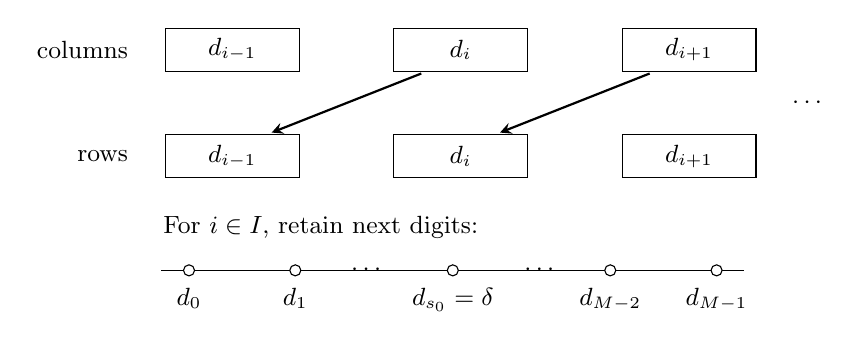
\begin{tikzpicture}[x=1cm,y=1cm,>=stealth,font=\small]
 \node[anchor=east] at (0,2.6) {columns};
 \node[anchor=east] at (0,1.25) {rows};
 \foreach \x/\lab in {1.2/{i-1},4.1/{i},7/{i+1}} {
   \node[draw,minimum width=1.7cm,minimum height=.55cm]
     at (\x,2.6) {$d_{\lab}$};
   \node[draw,minimum width=1.7cm,minimum height=.55cm]
     at (\x,1.25) {$d_{\lab}$};
 }
 \draw[->,thick] (3.6,2.3)--(1.7,1.55);
 \draw[->,thick] (6.5,2.3)--(4.6,1.55);
 \node at (8.5,1.93) {$\cdots$};
 \node[anchor=west] at (.2,.35)
   {For $i\in I$, retain next digits:};
 \draw (.3,-.2)--(7.7,-.2);
 \foreach \x/\lab in {.65/{d_0},2/{d_1},4/{d_{s_0}=\delta},6/{d_{M-2}},7.35/{d_{M-1}}} {
   \draw[fill=white] (\x,-.2) circle (2pt);
   \node[below] at (\x,-.3) {$\lab$};
 }
 \node at (2.9,-.2) {$\cdots$};
 \node at (5.1,-.2) {$\cdots$};
\end{tikzpicture}
\caption{One matching stage. Arrows show the first band of possible
pairings from a column cluster to the preceding row cluster; each
indicated cluster pair contains all lower-label pairs. In a retained
central cluster $i\in I$, the marked next digits have no pivot. The
spacings are schematic. The fixed-cut argument below uses the protected
digit $\delta=d_{s_0}$ to rule out crossings at sufficiently large
stages.}
\label{op:matching-figure}
\end{figure}

Fix now $J\in\Z$. At a sufficiently large stage, a possible matched
pair crossing $J$ would have column index
\[
 J<j\le J+X(1/M+2/p),
\]
since new matches occur only in the first band. Its lower label is
\[
 (\alpha+j)\bmod X=(X-1)/2+j
\]
without wrap, and its next digit is $\delta$. If the lower label is
eligible, its cluster index lies in $I$. In fact its representative
divided by $X$ differs from $1/2$ by at most
$1/M+2/p+o(1)$; if its last digit is $d_i$, the same representative
differs from $(i+1/2)/M$ by at most $1/p$. Hence $i$ is within three
places of $s_0$ for large $X$, which is inside $I$ since $M\ge81$.
But the next digit $\delta=d_{s_0}$ was explicitly retained there.
Such a pair cannot be matched. The remaining finitely many depths
each have only finitely many pairs crossing $J$. This proves the
first assertion.

For the second assertion, use labels with the prescribed units digit
and all later digits in $d(I)$ for columns or $d(I-1)$ for rows,
eventually all equal to $\delta$. These survive at every stage.
Changing finitely many digits of $\alpha$ gives an integer offset,
so each such label is $\alpha+j$ for a genuine integer row or
column index $j$. At a highest
modified position $r\ge1$, choose a center digit strictly below
$\delta$ for a column or strictly above it for a row. Both sets of
center digits contain such choices. The change at position $r$ has
absolute value at least $p^r$, while all lower changes together
have absolute value less than $p^r$, so this determines the
appropriate sign of the offset. The remaining $r-1$ intermediate digits can be
chosen freely, giving at least $B_0^{r-1}$ distinct offsets of
absolute value less than $p^{r+1}$. For $p^{r+1}\le N<p^{r+2}$,
these offsets lie in the required intervals and
\[
 B_0^{r-1}=p^{\beta(r-1)}\ge p^{-3\beta}N^\beta.
\]
Reducing the constant if necessary to work on both sides proves
the assertion for every sufficiently large integer $N$, including
cutoffs between successive powers of $p$.
\end{proof}
